\documentclass{standalone}
\usepackage{tikz}
\usepackage{float}
\usepackage{amsmath}
\usepackage{lmodern}
\usepackage{amssymb}
\usetikzlibrary{calc}
\usetikzlibrary{hobby}
\usetikzlibrary{decorations.markings}
\usetikzlibrary{patterns, patterns.meta}
\usetikzlibrary{shapes}

\begin{document}

\centering

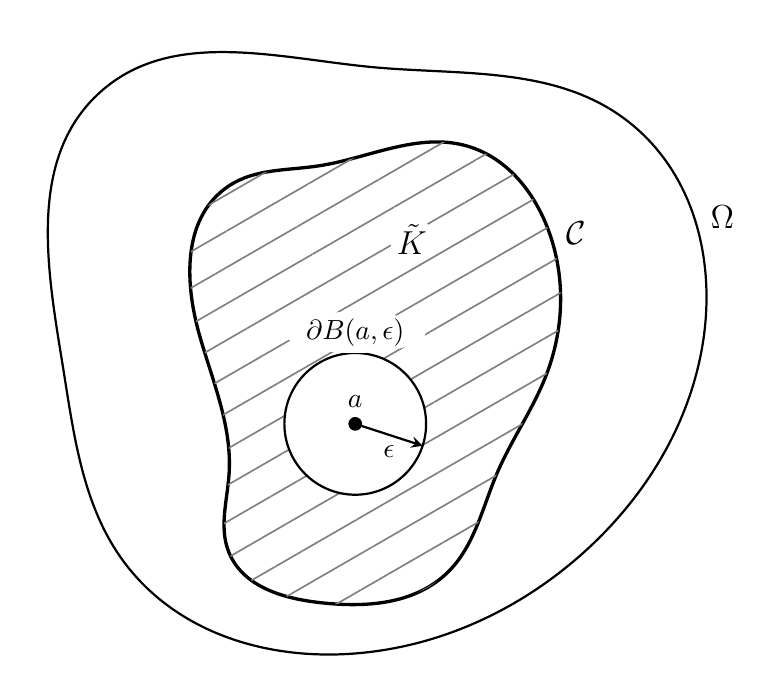
\begin{tikzpicture}[scale=0.9]
\pgfmathsetmacro{\CircleSize}{0.08}     % radius of coordinate circles/dots
% define styles used in this picture
\tikzset{
BigTextFont/.style={font=\large},
every node/.style={font=\normalsize, text=black},
CircleNodeStyle/.style={draw=black, shape=circle, fill=black, minimum size=\CircleSize*2 cm, inner sep=0pt},
arrowstyle/.style={->, >=stealth}}

% waypoint coordinates (in degrees, as seen from origin)
\begin{scope}[xshift = -3.0cm, yshift= -2.9cm, scale=1.8]
       \coordinate (OD) at (4.3,1);
       \coordinate (20D) at (5.2,2.5);
       \coordinate (40D) at (4.6,4.4);
       \coordinate (55D) at (2.6,4.8);
       \coordinate (80D) at (0.5,4.6);
       \coordinate (110D) at (0.2,2.5);
       \coordinate (300D) at (0.7,0.9);
       \coordinate (330D) at (2.5,0.2);
\end{scope}

% drawing area ("hobby" package)
\draw[postaction={decorate}, decoration={
       markings,
       mark=at position 0.17 with {\node[above right, BigTextFont] {$\Omega$};}}]
[thick] (OD) to[closed, curve through =
{(20D) (40D) (55D) (80D) (110D) (300D) }] (330D);

% CHECK
%plotting the waypoints
%\foreach \c in {(OD), (20D), (40D), (55D), (80D), (110D), (300D), (330D)} {
%       \fill[red] \c circle (1.0mm);
%       \node[above right] at \c {\c};
%}

% waypoint coordinates (in degrees, as seen from origin)
\begin{scope}[scale=1.4]
\coordinate (Odegrees) at (2.5,0);
\coordinate (20degrees) at (3,1);
\coordinate (40degrees) at (3,2.5);
\coordinate (55degrees) at (2.2,3.3);
\coordinate (80degrees) at (0.7,3.1);
\coordinate (95degrees) at (-0.2,2.9);
\coordinate (110degrees) at (-0.5,1.4);
\coordinate (180degrees) at (-0.2,0);
\coordinate (260degrees) at (-0.2,-0.8);
\coordinate (300degrees) at (0.7,-1.3);
\coordinate (330degrees) at (2.0,-1.0);
\end{scope}

\draw[postaction={decorate}, decoration={
       markings,
       mark=at position 0.17 with {\node[above right, BigTextFont] {$\mathcal{C}$};}}]
[very thick] (Odegrees) to[closed, curve through =
{(20degrees) (40degrees) (55degrees) (80degrees) (95degrees) (110degrees)  (180degrees) (260degrees) (300degrees) }] (330degrees);

% CHECK: turn on for plotting the waypoints
%\foreach \c in {(Odegrees),(20degrees),(40degrees),(55degrees),(80degrees),
%(95degrees),(110degrees),(180degrees),(260degrees),(300degrees),(330degrees)} \fill[red] \c circle (1.0mm);

% center of epsilon area
\coordinate (aLocation) at (1.5,0.7);   
\node [CircleNodeStyle, label=above:$a$] at (aLocation) {};

% fill the area (area must be copied here!), apply a clip for epsilon area
\begin{scope}
       \clip[overlay] (aLocation) circle [radius=1.0]
       (-20,-20) rectangle (30,20);
       \fill[pattern={Lines[angle=30, distance=0.4cm, line width=0.6pt]}, pattern color=gray] (Odegrees) to[closed, curve through ={(20degrees) (40degrees) (55degrees) (80degrees) (95degrees) (110degrees)  (180degrees) (260degrees) (300degrees) }] (330degrees);
       \end{scope}

% create epsilon area
\draw[thick] 
[postaction={decorate}, decoration={
       markings,
       mark=at position 0.25 with {\node[draw=white, ellipse, inner sep=0, fill=white, name=EndVectorNode, above] {$\partial B(a,\epsilon)$};},    % ensure node has a white background
       mark=at position 0.95 with {\node[name=EndVectorNode] {};}}]
(aLocation) circle [radius=1.0];

% draw radius of area
\draw[thick, arrowstyle]
[postaction={decorate}, decoration={
       markings,
       mark=at position 0.5 with {\node[name=EndVectorNode, below] {$\epsilon$};}}] 
(aLocation) -- (EndVectorNode.center);

% Compactum symbol
\coordinate (CompactumSymbolLoc) at (2.3,3.3);   
\node[draw=white, ellipse, inner sep=0, fill=white, name=EndVectorNode, BigTextFont] at (CompactumSymbolLoc) {$\tilde K$};

\end{tikzpicture}

\end{document}